\documentclass{beamer}

\usepackage{hyperref}
\usepackage{listings}

\title{Automatic calculation of plane loci using Groebner bases and integration into a Dynamic Geometry System}   
\author{Michael Gerh\"auser, Alfred Wassermann} 
\date{July 24, 2010} 

\newcommand{\GEONEXT}{GEONE\kern-.06em \lower.5ex\hbox{x}\kern-.215em T}
\definecolor{GXT}{rgb}{0,0.549019608,0}
\setbeamercolor{title}{fg=GXT}
\setbeamercolor{frametitle}{fg=GXT}
\setbeamercolor{blocktitle}{fg=GXT}
\setbeamercolor{section in toc}{fg=GXT}
\usebackgroundtemplate{
\includegraphics[width=\paperwidth]{img/background.png}}
\logo{
\includegraphics[height=0.75cm]{img/ubt.png}}
\beamertemplatenavigationsymbolsempty

\begin{document}

\frame{\titlepage} 

\frame{\frametitle{Overview}\tableofcontents}

\section{JSXGraph - A short overview} 

% JSXGraph

\frame{
  \frametitle{}

  \begin{block}{JSXGraph}
  \end{block}
}

\frame{
  \frametitle{JSXGraph}

  \begin{block}{What is JSXGraph?}
    \begin{itemize}
      \item A library implemented in JavaScript
      \item Runs in recent versions of all major browsers
      \item No plugins required
      \item LGPL-Licensed
    \end{itemize}
  \end{block}

  \begin{block}{Main features}
    \begin{itemize}
      \item Dynamic Geometry
      \item Interactive function plotting
      \item Turtle Graphics
      \item Charts
    \end{itemize}
  \end{block}
}

\frame{
  \frametitle{JSXGraph} 
  \begin{block}{Supported Hardware}
    \begin{itemize}
      \item PC (Windows, Linux, Mac)
      \item Mobile phones
      \item "Touchpads" like the Apple iPod and iPad
      \item Basically everything which runs at least one of the supported browsers
    \end{itemize}
  \end{block}
}

\frame{
  \frametitle{JSXGraph} 
  \begin{block}{Supported Browsers}
    \begin{itemize}
      \item Firefox
      \item Chrome/Chromium
      \item Safari
      \item Internet Explorer
      \item Opera
    \end{itemize}
  \end{block}
}

\lstset{ %
language=Java,                % choose the language of the code
basicstyle=\tiny,       % the size of the fonts that are used for the code
numbers=none,                   % where to put the line-numbers
numberstyle=\footnotesize,      % the size of the fonts that are used for the line-numbers
stepnumber=1,                   % the step between two line-numbers. If it's 1 each line 
                                % will be numbered
numbersep=5pt,                  % how far the line-numbers are from the code
backgroundcolor=\color{white},  % choose the background color. You must add \usepackage{color}
showspaces=false,               % show spaces adding particular underscores
showstringspaces=false,         % underline spaces within strings
showtabs=false,                 % show tabs within strings adding particular underscores
frame=single,	                % adds a frame around the code
tabsize=2,	                % sets default tabsize to 2 spaces
captionpos=b,                   % sets the caption-position to bottom
breaklines=true,                % sets automatic line breaking
breakatwhitespace=false,        % sets if automatic breaks should only happen at whitespace
title=\lstname,                 % show the filename of files included with \lstinputlisting;
                                % also try caption instead of title
escapeinside={\%*}{*)},         % if you want to add a comment within your code
morekeywords={*,...},           % if you want to add more keywords to the set
morestring=[d][\color{blue}]{'},
morecomment=[s][\color{gray}]{<}{>},
morecomment=[s][\itshape\color{gray}]{[.}{.]}
}

\begin{frame}[fragile]
  \frametitle{JSXGraph} 
  \begin{block}{Example/Input}
    \begin{lstlisting}
<link rel="stylesheet" type="text/css" href="css/jsxgraph.css" />
<script type="text/javascript" src="js/jsxgraphcore.js"></script>
[...]
<div id="jxgbox" class="jxgbox" style="width:500px; height:500px;"></div>
<script type="text/javascript">
  /* <![CDATA[ */
  board = JXG.JSXGraph.initBoard('jxgbox', {boundingbox: [-2, 20, 20, -2], axis: true, grid: false, keepaspectratio: true, showcopyright: false});
  p3 = board.create('point', [8, 3]);
  p4 = board.create('point', [8, 8]);
  c1 = board.create('circle', [p4, 4]);
  p6 = board.create('glider', [0, 0, c1], {name: 'D'});
  g = board.create('line', [p3, p6]);
  c2 = board.create('circle', [p6, 3]);
  p14_1 = board.create('intersection', [c2,g,0], {name: 'T'});
  /* ]]> */
</script>
    \end{lstlisting}
  \end{block}
\end{frame}

\frame{
  \frametitle{JSXGraph}

  \begin{block}{Example/Output}
\begin{center}
      \href{http://localhost/~michael/jxg/examples/adg/limacon.html}{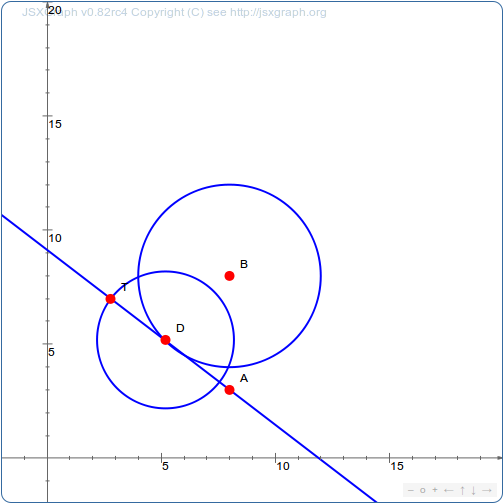
\includegraphics[width=5cm]{img/jsx-example.png}}
\end{center}
  \end{block}
}


% Groebner bases stuff

\section{Computing plane loci using Groebner bases}

\frame{
  \frametitle{}

  \begin{block}{Computing plane loci using Groebner bases (in a nutshell)}
  \end{block}
}

\frame{
  \frametitle{Computing plane loci using Groebner bases}

  \begin{block}{}
    \begin{itemize}
      \item Given a set of free and dependent points,
\begin{center}
      \href{http://localhost/~michael/jxg/examples/adg/limacon.html}{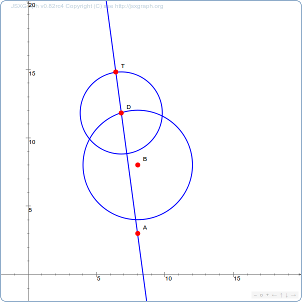
\includegraphics[width=5cm]{img/limacon-base.png}}
\end{center}
    \end{itemize} 
  \end{block}
}

\frame{
  \frametitle{Computing plane loci using Groebner bases}

  \begin{block}{}
    \begin{itemize}
      \item we first choose a coordinate system,
\begin{center}
      \href{http://localhost/~michael/jxg/examples/adg/limacon.html}{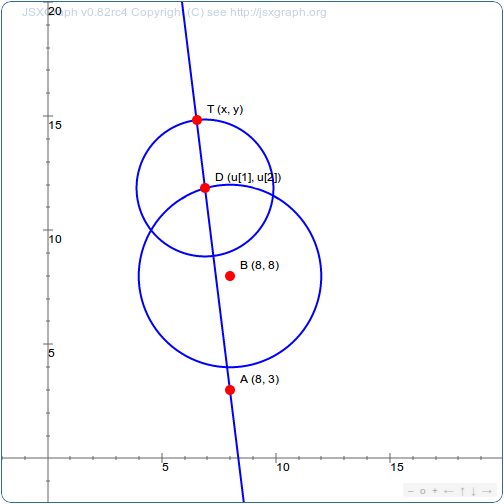
\includegraphics[width=5cm]{img/limacon-coords.png}}
\end{center}
    \end{itemize} 
  \end{block}
}

\frame{
  \frametitle{Computing plane loci using Groebner bases}

  \begin{block}{}
    \begin{itemize}
      \item translate geometric constraints into an algebraic form,
\begin{itemize}
  \item $(u[1]-8)^2 + (u[2]-8)^2 - 16 = 0$
  \item $(x-u[1])^2 + (y-u[2])^2 - 9 = 0$
  \item $3x-3u[1]+yu[1]-8y+8u[2]-xu[2] = 0$
\end{itemize}
    \end{itemize} 
  \end{block}
}

\frame{
  \frametitle{Computing plane loci using Groebner bases}

  \begin{block}{}
    \begin{itemize}
      \item calculate the Gr\"obner basis of the given ideal,
\begin{itemize}
  \item $x^6+3x^4y^2+3x^2y^4+y^6-48x^5-38x^4y-96x^3y^2-76x^2y^3-48xy^4-38y^5+1047x^4+1216x^3y+1774x^2y^2+1216xy^3+727y^4-13024x^3-16596x^2y-16096xy^2-8404y^3+97395x^2+109888xy+63535y^2-415536x-300806y+790009 = 0$
\end{itemize}
    \end{itemize} 
  \end{block}
}

\frame{
  \frametitle{Computing plane loci using Groebner bases}

  \begin{block}{}
    \begin{itemize}
      \item and finally plot the calculated implicit equation.
\begin{center}
      \href{http://localhost/~michael/jxg/examples/adg/limacon.html}{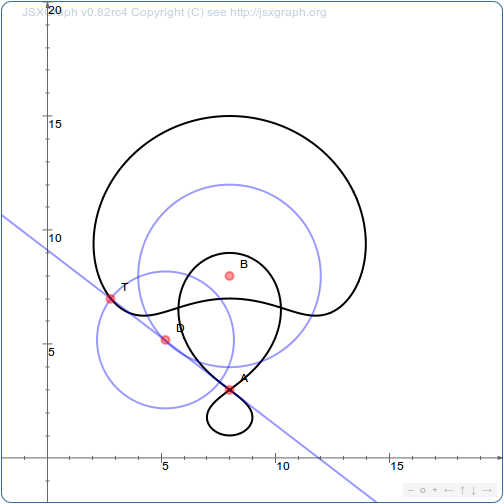
\includegraphics[width=5cm]{img/limacon-locus.png}}
\end{center}
    \end{itemize} 
  \end{block}
}

\section{Implementing this algorithm in JSXGraph}

\frame{
  \frametitle{}

  \begin{block}{Implementing this algorithm in JSXGraph}
  \end{block}
}

\frame{
  \frametitle{Implementing this algorithm in JSXGraph}

  \begin{block}{Problems}
    \begin{itemize}
      \item No JavaScript implementation of any Gr\"obner basis algorithm
      \item Can't use C-libraries directly in JavaScript
      \item No implicit plotting in JSXGraph by now
    \end{itemize}
  \end{block}
}

\frame{
  \frametitle{Implementing this algorithm in JSXGraph}

  \begin{block}{Our solution}
    \begin{itemize}
      \item XMLHttpRequest/AJAX to 
    \end{itemize}
  \end{block}
}

\section{Optimizations}

\frame{
  \frametitle{}

  \begin{block}{Optimizations}
  \end{block}
}

\section{Examples}

\frame{
  \frametitle{}

  \begin{block}{Examples}
  \end{block}
}

\end{document}
